
\documentclass[10pt,journal,compsoc]{IEEEtran}
\usepackage{listings}
\usepackage[pdftex]{graphicx}    
\usepackage{cite}
\hyphenation{op-tical net-works semi-conduc-tor}


\begin{document}

\title{Elegant Racer-bot}

\author{Myoungki Jung}

\markboth{Localization project, Robotics Nanodegree Program, Udacity}%
{}
\IEEEtitleabstractindextext{%

\begin{abstract}
A localisation of robots is a key requirments task management for autonomous robots. Its implementation in robotics operating system provides a good starter point entering this topic.
The purpose of this report is to show the application of off the shelf localisation package inin a simulated condition, robotics operating system(ROS), its implementation, tunning parameters and results.
\end{abstract}

% Note that keywords are not normally used for peerreview papers.
\begin{IEEEkeywords}
Robot, IEEEtran, Udacity, AMCL, ROS, Localization, Racer.
\end{IEEEkeywords}}


\maketitle
\IEEEdisplaynontitleabstractindextext
\IEEEpeerreviewmaketitle
\section{Introduction}
\label{sec:introduction}

\IEEEPARstart{T}{he} localisation is a classic robotics topic with a long history and many variation. Localisation is a task with this question in mind continously.
'Where am I?' In addition, the result of localisation, space or position, is a major domain which compose of a task.
Without knowing the position of an actor, the actor cannot perform any designated task in a place. To perform a task delegated to an actor, knowing the location is a essential step and the accuracy of the evaluation also influences the success of the task greatly.
To carry out a sucessful localisation, kalman filters and a monte carlo localisation algorithm will be used from the robotics operating system packages, instead of implementing the algorithm from source code.
Wihtout positioning the robot to a desired area no other subsuent action can take place in it. Therefore, correct parameters from an adequate tuning process, a high accuracy of pose estimation will be given and this allows other tasks robot performing as intended. However, derieving a set of optimised parameter requires much knowledge on the software package, observation skill, and scientific decisions.

\section{Background}

\subsection{Kalman Filters}
Kalman filters are used in evaluation of real value from sensors with noises. Extended Kalman Filter(EKF) is prferred when the filtered data is passed to a monte carlo localisation becuase normal linear kalman filter does not allow nonlinear transformation function, and monte carlo localisation allows computation of non linear functions. 
Filteration with an extended kalman filter is a crucial action before inserting the sensor data into a localisation process pipe line as the errors in raw sensor values can propagate and amplify its magnitude greater later in localisation processes.
Therefore, filteration of noise and evaluation of near true value ensure the overall accuracy of the localisation.
\subsection{Particle Filters}
Particle filters is a common localisa     tion tool
Normal monte carlo localisation algorithm is shown in \ref{fig:mcl_algo}. 
\begin{figure}[thpb]
      \centering
      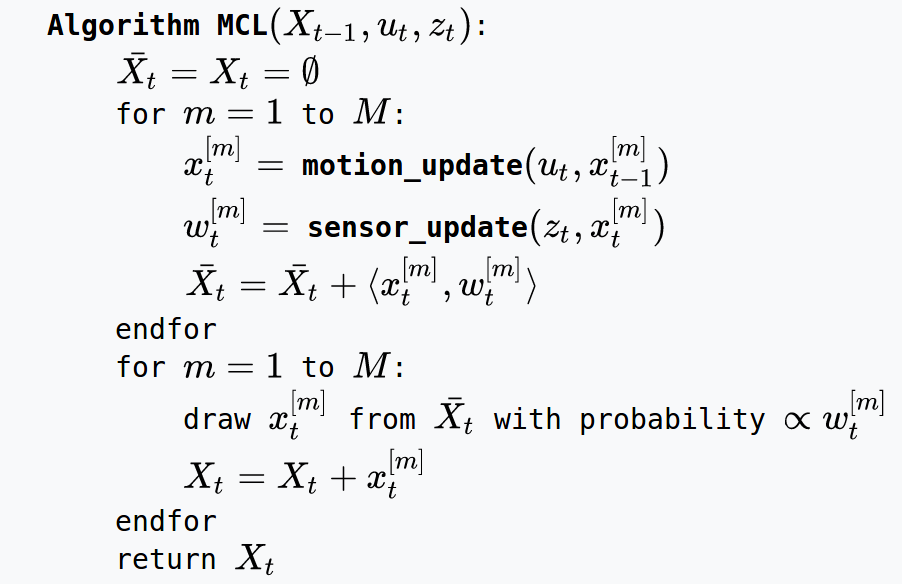
\includegraphics[width=\linewidth]{./img/mcl_algo.png}
      \caption{Algorithm of Monte Carlo localization}
      \label{fig:mcl_algo}
      \cite{Thrun2002}
\end{figure}
Adaptive (or KLD-sampling) Monte Carlo localization (AMCL)is a probabilistic localization method for a robot being position on two dimensions.\cite{Fox2001}.
KLD sampling reduced computation load by probabilistic sampling in a error range.\cite{Fox2001} This increases the performance of system performing MCL, allowing low end comuters acheive higher rate of MCL evaluation.
Allowance of algorithms to low power machines is a important trend for mobile robots recently.

\subsection{Comparison / Contrast}

The Table \ref{table:comparison_ekf_mcl} shows the comparision bewteen the extended kalman filter and monte carlo localisation in various features.
\begin{table}[ht]
      \caption{EKF vs. MCL}
      \label{table:comparison_ekf_mcl}
      \begin{center}
      \begin{tabular}{|c|c|c|}
      \hline
       & MCL & EKF \\
      \hline\hline
      Measurement types & Raw & Landmark \\
      \hline
      Measurement Noise & Any &  Gaussian \\
      \hline
      Posterior & Particles &  Gaussian \\
      \hline
      Memory Efficiency & Normal &  Good \\
      \hline
      Time Efficiency & Normal &  Good \\
      \hline
      Code difficulty & Easy &  Normal \\
      \hline
      Resolution & Normal &  Good \\
      \hline
      Robustness & Good &  No \\
      \hline
      Memory \& resolution & Yes &  No \\
      \hline
      Global localisation & Yes &  No \\
      \hline
      State space & Multimodal discrete &  Unimodal continous \\
      \hline
      \end{tabular}
      \end{center}
\end{table}


Kalman filters and particle filters can make synergy in performance and accuracy.  For a mobile robot in 2D, kalman filter can be used in embedded sensors to output less noise sensor readings to the main processing unit, and particle filters in main processing unit can utilise the noiseless sensor values to evaluate the position of the system.

\section{Simulations}
This section should discuss the performance of robots in simulation. Items to include are the robot model design, packages used, and the parameters chosen for the robot to properly localize itself. The information provided here is critical if anyone would like to replicate your results. After all, the intent of reports such as these are to convey information and build upon ideas so you want to ensure others can validate your process.
You should have at least two images here: one that shows your standard robot used in the first part of the project, and a second robot that you modified / built that is different from the first robot. Remember to watermark all of your images as well. 

\subsection{Achievements}
You should describe what you achieved for localization in the project with the benchmark model and your own model. Includes charts and graphs show how parameters affect your performance. 

% Robot Models
\subsection{Benchmark Model}
\subsubsection{Model design}
the layout and used sensors are shown in Table \ref{table:model_design}.
\begin{table}[ht]
      \caption{Model Design}
      \label{table:model_design}
      \begin{center}
      \begin{tabular}{|c|c|}
      \hline
      Atribute & Value \\
      \hline\hline
      \hline
      Size & 0.15 m by 0.10 m \\
      \hline
      Camera & Generic RGB  \\
      \hline
      LIDAR & Hokyuo  \\
      \hline
      \end{tabular}
      \end{center}
\end{table}
\subsubsection{Packages Used}
The packages used in the project should be specified as well as the topics received and published; the services it used and provided should also be addressed. 
\subsubsection{Parameters}
Localization parameters in the AMCL node should be described, as well as move\_base parameters in the configuration file. You should be able to clearly demonstrate your understanding of the impact of these parameters.


\subsection{Personal Model}
\subsubsection{Model design}
The design of the model is the same as the udacity model. This was intended as offline vehicle for this simulation is sparkfun rebot(Figure \ref{fig:sparkfunredbot}).
The realsense camera D435 was intended to use in the model the package in githubs were obsolete and did not work with the project well.

\begin{figure}[thpb]
      \centering
      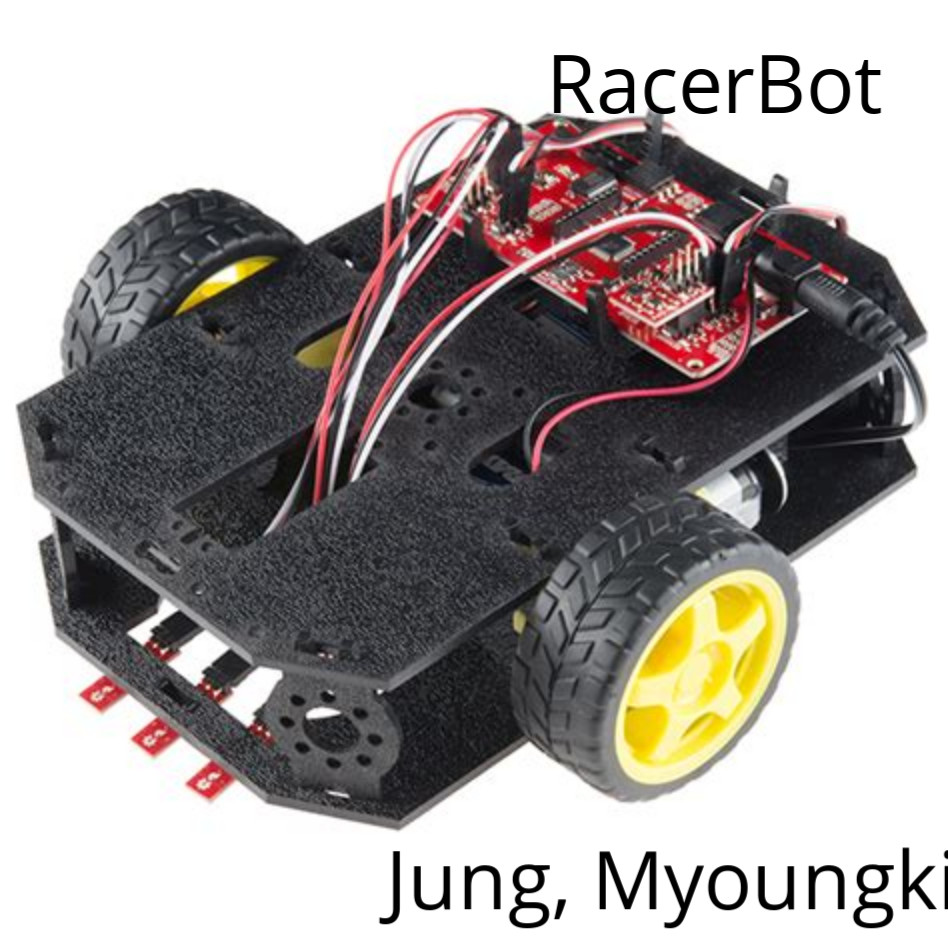
\includegraphics[width=\linewidth]{./img/sparkfunredbot.jpeg}
      \caption{Sparkfun Redbot}
      \label{fig:sparkfunredbot}
\end{figure}
\subsubsection{Packages Used}
In the simulation the same sensor was used, however, in offline model will have two proximity sensors or a generic sweeping LIDAR instead of hokyuo 1D LIDAR.

\subsubsection{Parameters}

\begin{lstlisting}[language=Python, caption=Fully convolutional network code]
def fcn_model(inputs, num_classes):

      filter= 32
      
      return filter
\end{lstlisting}

%example for Bullet point list
\begin{itemize}
      \item example 1
      \item example 2
      \end {itemize}
      
      %example for numbered list
      \begin{enumerate}
      \item example 1
      \item example 2
      \end{enumerate}

\section{Results}
Present an unbiased view of your robot's performance and justify your stance with facts. Do the localization results look reasonable? What is the duration for the particle filters to converge? How long does it take for the robot to reach the goal? Does it follow a smooth path to the goal? Does it have unexpected behavior in the process? \\
For demonstrating your results, it is incredibly useful to have some watermarked charts, tables, and/or graphs for the reader to review. This makes ingesting the information quicker and easier.
\subsection{Localization Results}

The Figure \ref{fig:goal_arrival} shows the robot can reach the goal by itselft. The pose array is densely populated right infront of the robot, not on the centre of inertia. However, this does not cause any trouble in navigation and collision avoidance.
\begin{figure}[thpb]
      \centering
      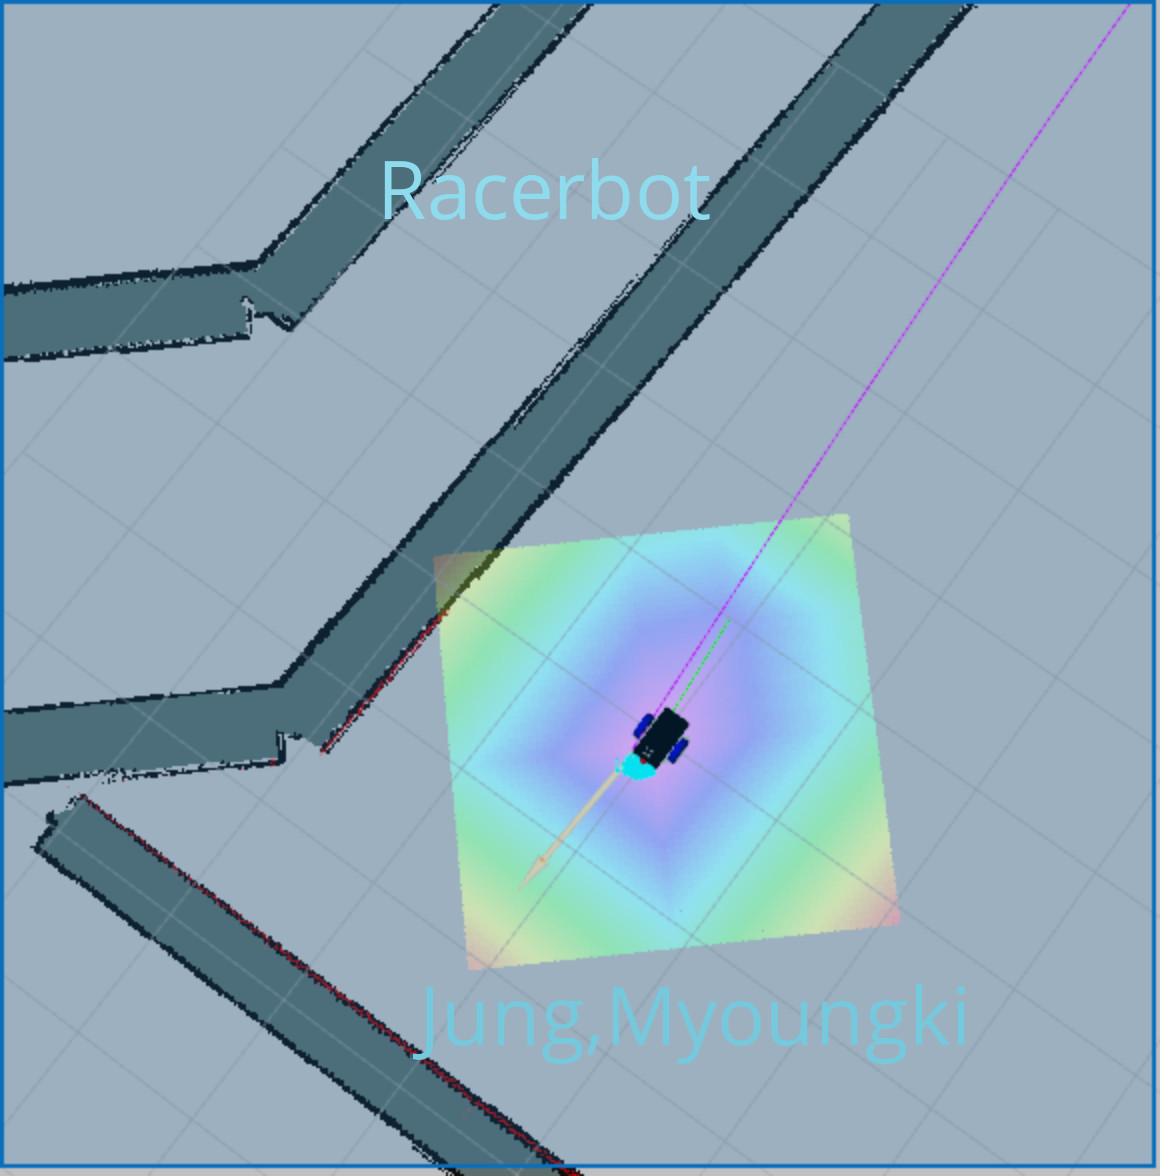
\includegraphics[width=\linewidth]{./img/goalarrival.png}
      \caption{Arrival to the goal}
      \label{fig:goal_arrival}
\end{figure}
The orange arrow represents the current goal pose, the violet line is the NavFPath of ROS, a short green line is the local path, and the rainbow box shows the coloured heat map of total cost. 
The Figure  \ref{fig:goalconsole} shows that the robot arrived to the 
\begin{figure}[thpb]
      \centering
      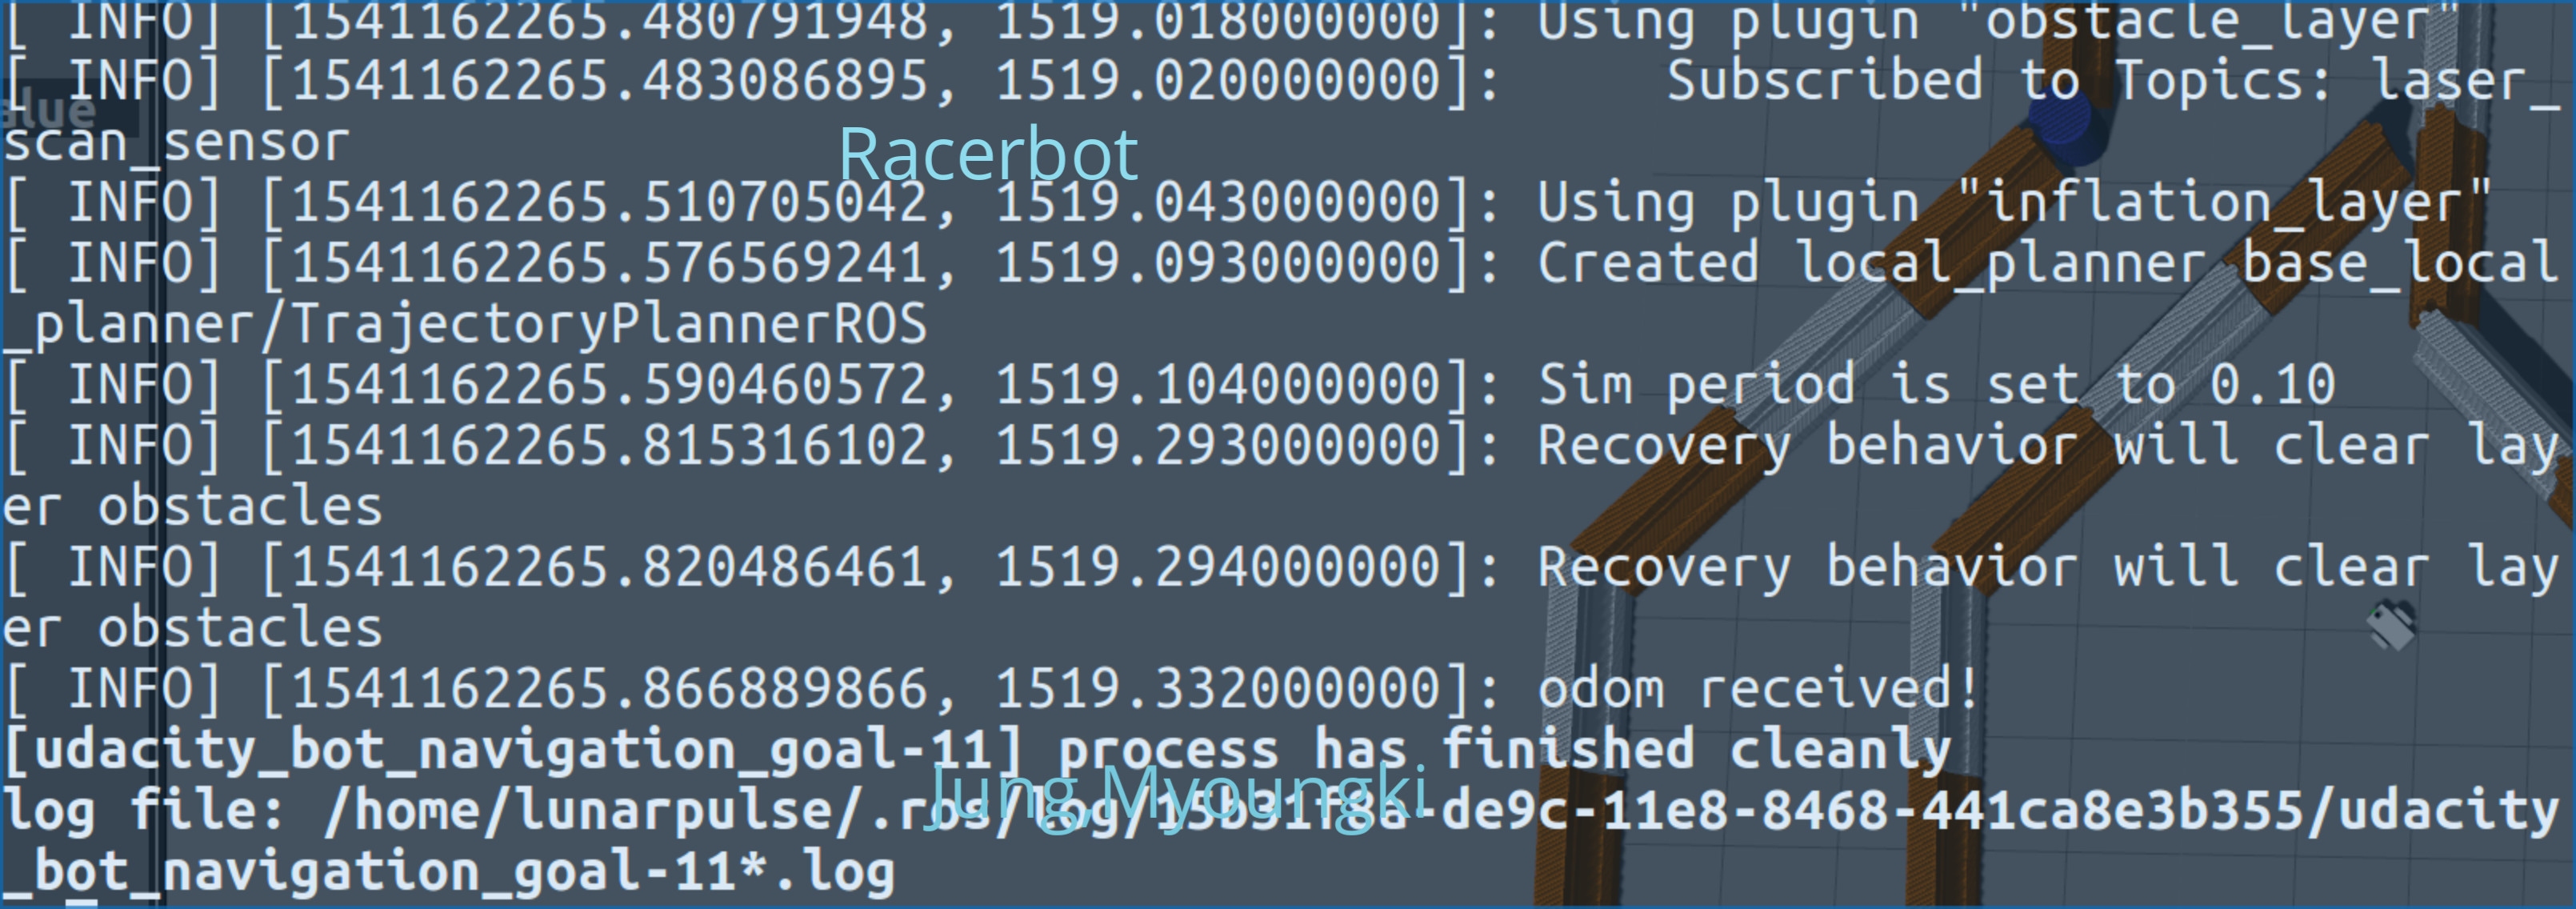
\includegraphics[width=\linewidth]{./img/goalconsole.png}
      \caption{Arrival to the goal}
      \label{fig:goalconsole}
\end{figure}
In the figure, local cost map is relatively flat because no obstacles inside the local cost map because The total cost function is dependent on the sensored obstacles and the certainty of mcl localisation and the result cost map becomes indifferent. 
Figure \ref{fig:localcostmap} shows the local cost map with an array of obstacle in the scene, the contour of cost map is more steep and shows the prefered heading of the robot as bright purple, red is the opposite direction. In addition, there is a slight descripency between local path and global navigation path. the robot is following in between two path, and sometimes runs off the route before and after a narrow curve. The Figure \ref{fig:localcostmap} shows a recovery of its heading from a U-turn.
\begin{figure}[thpb]
      \centering
      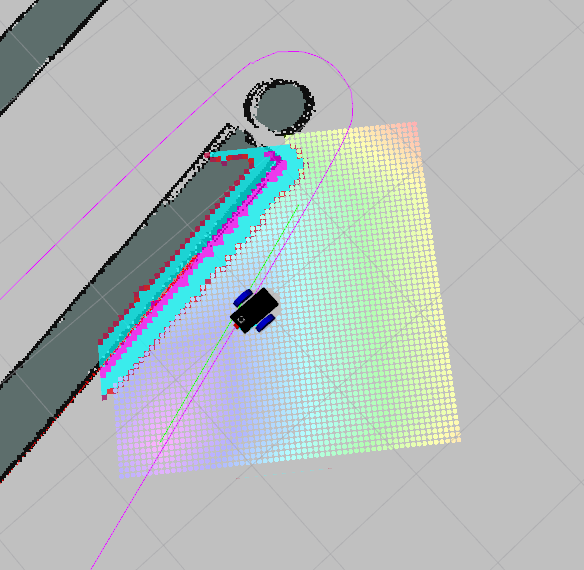
\includegraphics[width=\linewidth]{./img/localcostmap.png}
      \caption{Local cost map with obstacle existing on one side}
      \label{fig:localcostmap}
\end{figure}
\subsubsection{Benchmark}
\subsubsection{Student}


\subsection{Technical Comparison} % only facts
Discuss the difference of the layout, parameters, performance etc. between the benchmark robot and your robot. It is acceptable for your custom robot to perform worse than the provided robot. The focus is on learning and understanding, not performance. 

\section{Discussion}

The localisation provided by the AMCL was intuitive and provided a successful localisation with small variance was achieved with the default values for its parameters. It is an easy use of the adaptive monte carlo localisation. The scattered arrows of estimated poses were gathered to the model of the robot in 5 seconds while navigating between the obstacles due to the observed obstacles in a continous manner, if it was in a place without any obstacles in a detectable range of the sensor, it takes a longer time to pin the pose of the robot. The cost cloud map also is related to the existance of local obstacles too.

The local cost map becomes indifference when the robot enters in a area without any obstacle in its sernsoring area. The contour of the cost map become flatter and the navigation stack started to make oscilation becuase the local goal is spreaded and not obvious to take. In some areas robot roams randomly or make arcs instead of following the planned path. This issue was solved by increasing the pDist twice more than gDist(default value 0.8). With pDist (3.5) and and gDist (1.5) robot tends to follow the global goal more than being lost in an uncertain local plan. This also was tweaked by the maximum speed of the robot in later section.

With robot radious 0.0 or not defined, the robot tends to hit to the corner, as the path planner provides very tight corners which is surely the optimised or the shortest path. However, with out the robot radious parameter tuned robot hits to the pillar and slows down by drawing arcs around it. In addition, top speed of the robot set to 0.5, this was entirely solved and shows a easy cornering without touching the corners.

The resolution of the local cost map was set to 0.05. A higher value, more than 0.1 gave a coarse representation of action and cost anaylysis and rendered the robot roaming indecisively. However, the lower value resulted a flat, less gradient between contours of cost in the grid, and this also affected the behaivour of the robot in a similar manner with the higher value. 


\subsection{Topics}
\begin{itemize}
\item Which robot performed better?
\item Why it performed better? (opinion)
\item How would you approach the 'Kidnapped Robot' problem?
\item What types of scenario could localization be performed?
\item Where would you use MCL/AMCL in an industry domain?
\end {itemize}

\section{Conclusion / Future work}
This section is intended to summarize your report. Your summary should include a recap of the results, did this project achieve what you attempted, how would you deploy it on hardware and how could this project be applied to commercial products? 

The set of technology used in this project can apply to many fields operating on the ground with two wheels. Robot vaccum cleaners have the same sets of sensors and actuators except, the vaccum device and continers. This two wheeled mobile platform with accurate localisation can be used as the base vehicle or carrier for many different research too. The callenges in implementation of this platfrom from a simulation to the offline is to select actuators, and its control logic, to program the interface firmware to the control logic and to build and tune according to the hardware specification iteratively.

Porting the simulation to a real robot has challenges. The calculation of inertia of the real physical body of the robot, instead of assumming all axis of inertia is 0.1. This will influence the parameters of costmap as the acceleration and deceleration of the offline robot will be different from the simulation, not only the calculation of the inertia, the noise level from the sensor will vary depending on the operational condition, EKF needs to be taking it accounted.

Overall, processes of tuning consumed majority of time and the amount of effort to understand the dynamics among navigation, localisation, and physics of robot was considerable in developing this even tough refering to the guide. With growing popularity of machine learning, the reinforcement learning is considered to be the very topic which can substitute human tunner's effort with probablistic analysis of parameters and acheive higher performance in a short time. This was shown by alpha go zero, mastering condensed human knowledge of Go for 2000 years  practice in a week. With new or continously changing systems, assumming no prior knowledge or short time expiry knowledge, such model free reinforcement leanring should be more approperiate to apply than relying human effort, as human tends to make mistakes in those situation.


\subsection{Modifications for Improvement}
Examples:
\begin{itemize}
\item Base Dimension
\item Sensor Location
\item Sensor Layout
\item Sensor Amount
\end{itemize}

\subsection{Hardware Deployment}
\begin{enumerate}
\item What would need to be done?
\item Computation time/resource considerations?
\end{enumerate}

\bibliography{bib}
\bibliographystyle{ieeetr}

\end{document}
